\maketitle
\setcounter{page}{1}
\tableofcontents
\newpage
\pagenumbering{arabic}
\section{Theorie}
Ziel des Versuchs ist die Untersuchung der Temperaturabhängigkeit des glühelektrischen
Effektes an einer Hochvakuumdiode. Als glühelektrischen Effekt wird die Emission von Elektronen aus einem
aufgeheizten Metall bezeichnet. Dabei muss an den Elektronen die sogenannte
Austrittsarbeit geleistet werden. Zur Erklärung dieses Begriffs ist die Vorstellung
des Metalls als Potentialtopf sinnvoll. Die positiv geladenen Kerne sind an einem
Gitter gebunden, das Potential der Kerne erzeugt einen Potentialtopf, der um $\phi$
vom umgebenden Potential abweicht. In diesem
Topf können sich die Elektronen frei bewegen, sie sind nicht mehr an ein Atom gebunden.
Um den Potentialtopf verlassen zu können, müssen die Elektronen mindestens dieses Potential
überwinden. Diese Überlegung führt zusammen
mit einigen Kentnissen über das Verhalten der Elektronen in ihrem Phasenraum auf die
$\textsc{Richardson}$-Gleichung
\begin{equation}
  j_{\symup{S}}(T) = 4 \pi \frac{e_0 m_0 k^2}{h^3} T^2 \exp\left(\frac{-e_0 \phi}{k T} \right),
  \label{eq:3}
\end{equation}
mit der aus der Temperatur $T$ sowie den Konstanten $e_0$ (Elementarladung),
$m_0$ (Elektronenruhemasse), $k$ ($\textsc{Bolzmann}$-Konstante) und
$h$ ($\textsc{Planksches}$ Wirkungsquantum) die Sättigungsstromdichte, also den Strom der Elektronen
aus der Metalloberfläche, berechnet werden.\\
\begin{figure}
  \centering
  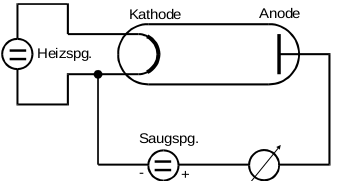
\includegraphics[scale=0.4]{hvdiode.png}
  \caption{Aufbau einer Hochvakuumdiode mit Heizkreislauf\cite{anleitung}.}
  \label{abb:5}
\end{figure}
Versuchsanordnungen zur Messung dieses Zusammenhanges schließen zwangsläufig ein
Vakuum ein, um Wechselwirkungen zwischen emittierten Elektronen und Umgebung zu verhindern.
Zusätzlich wird in ihnen ein elektrisches Feld angelegt, um die ungerichtete Elektronenemission
zu fokussieren. Dafür wird eine Anode in die Anordnung gebracht, die emittierende Metalloberfläche
dient als Kathode. Die Elektronen bewegen sich also nach ihrer Emission auf die Anode zu.
Einen solchen Aufbau bezeichnet man als Hochvakuumdiode (siehe Abbildung \ref{abb:5}). Bei Nutzung einer solchen
Anordnung wird jedoch festgestellt, dass der an der Anode gemessene Strom von der Spannung
der Anode abhängt und erst ab einer Sättigungsspannung $I_{\symup{S}}$ alle Elektronen die Anode erreichen.
Grund dafür ist die Beschleunigung, die die Elektronen im elektrischen Feld erfahren.
Die Ladungsdichte $\rho$ im Inneren der Diode ist somit Ortsabhängig. Als Konsequenz der
Kontinuitätsgleichung
\begin{equation}
  j = - \rho v
\end{equation}
wird das elektrische Feld nahe der Kathode sehr schwach, da es von
den austretenden Elektronen abgeschirmt wird. Die nachströmenden Elektronen können
die Anode dann nicht mehr erreichen. Der an der Anode gemessene Strom kann sich
also nur an den Sättigungsstrom annähern. Aus der $\textsc{Poisson}$-Gleichung
und der Energieerhaltung folgt für den Verlauf der Stromdichte in der Diode:
\begin{equation}
  j = \frac{4}{9} \varepsilon_0 \sqrt{2 e_0 / m_0} \frac{a^2}{V^{3/2}},
  \label{eq:4}
\end{equation}
das sogenannte $\textsc{Langmuir-Schottkysche}$ Raumladungsgesetz. $a$ bezeichnet dabei
die $x$-Position der Anode.\\
Aus \eqref{eq:4} folgt, dass ohne anliegendes Potential ($V \le 0$) kein Anodenstrom messbar ist.
In der Realität lässt sich aufgrund der Geschwindigkeit, die die Elektronen auch ohne
anliegende Spannung besitzen, ein gewisser Strom messen. Dieser Strom wird Anlaufstrom
genannt. Die Energie der Elektronen muss jedoch auch groß genug sein, ein äußeres
Potential $V$ zu überwinden. Allgemein gilt für die Anlaufstomstärke:
\begin{equation}
  j(V) = j_0 \exp\left(-\frac{e_0 \phi_A + e_0 V}{kT}\right),
  \label{eq:5}
\end{equation}
wobei $\phi_A$ die Austrittsarbeit des Anodenmaterials bezeichnet, die ebenfalls
überwunden werden muss.\\
Die Kombination der durch \eqref{eq:5}, \eqref{eq:4} und \eqref{eq:3} beschriebenen Abhängigkeiten
liefern die sogenannte Kennlinie der Hochvakuumdiode. Ohne anliegende Spannung kann nur
ein Anlaufstrom gemessen werden. Wird die Spannung erhöht, wird die $V^{3/2}$-Abhängigkeit
des Raumladungsgesetzes gemessen. Steigt die Spannung weiter, so strebt der gemessene Anodenstrom gegen
einen Sättigungswert. Ein Beispiel für eine Kennline bei konstantem $T$ ist in \ref{abb:6}
gegeben.
\begin{figure}
  \centering
  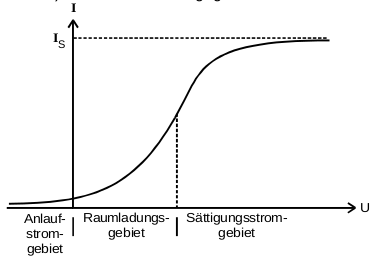
\includegraphics[scale=0.4]{kennlinie.png}
  \caption{Beispielhafte Kennline mit Kennzeichnung der einzelnen Abschnitte\cite{anleitung}.}
  \label{abb:6}
\end{figure}
\section{Durchführung}
\subsection{Versuchsaufbau}
Zur Bestimmung von Kennlinien wird ein Konstantspannungsgerät mit regelbaren Spannungen
zwischen Anode und Kathode geschaltet. Die in diesem
Kreislauf anliegenden Spannungen und Stromstärken werden über Messgeräte gemessen.
In einem zweiten Kreislauf wird an der Kathode ein Konstantspannungsgerät zur Erzeugung
der Heizspannung angeschlossen. Auch hier wird die Spannung gemessen (siehe \ref{abb:7}).
Für die Messung der Anlaufstromkurve wird eine abgewandelte Version dieser Schaltung
verwendet. Das Spannungsmessgerät des Anode-Kathode
Kreislaufs wird entfernt, die Spannungsquelle wird umgepolt und durch ein Konstantspannungsgerät
im \SI{1}{\volt} Bereich ersetzt. Das Amperemeter wird durch eines mit Messbereich im \si{\nano\ampere}
Bereich ersetzt (siehe \ref{abb:8}).
\begin{figure}
\centering
  \begin{subfigure}{0.4\textwidth}
    \centering
    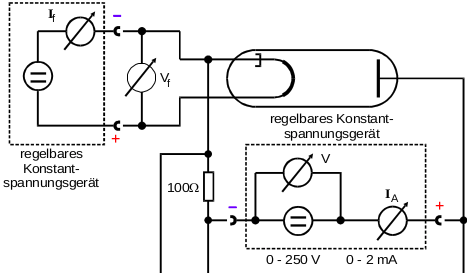
\includegraphics[width=\textwidth]{aufbken.png}
    \caption{Versuchsaufbau zur Bestimung von Kennlinen. Grafik wurde
    den tatsächlichen Gegebenheiten angepasst\cite{anleitung}.}
    \label{abb:7}
  \end{subfigure}
  \begin{subfigure}{0.4\textwidth}
    \centering
    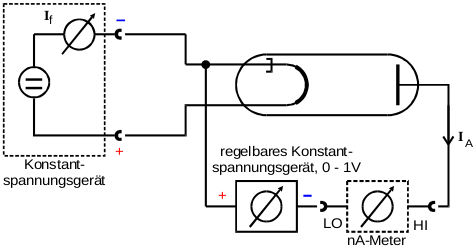
\includegraphics[width=\textwidth]{aufbanl.png}
    \caption{Versuchaufbau zur Bestimmung des Anlaufstroms\cite{anleitung}.}
    \label{abb:8}
  \end{subfigure}
  \caption{Übersicht über die Versuchsaufbauten.}
\end{figure}
\subsection{Versuchsdurchführung}
In einem ersten Versuchsteil wird die Temperaturabhängigkeit des Sättigungsstroms ermittelt.
Dazu werden für verschiedene Heizspannungen die Spannung in \SI{10}{\volt} Schritten
erhöht und die Stromstärke abgelesen.
Die erzeugte Temperatur wird jewils aus der Leistungsbilanz des Heizkreislaufs bestimmt.
Daraus wird dann die Austrittsarbeit der Kathode bestimmt.
In einem folgenden Versuchsteil wird für die maximale Heizspannung
aus einer Kennline der Gültigkeitsbereich von \eqref{eq:4} ermittelt und der
Tatsächlie Exponent der $V$-Abhängigkeit bestimmt. Desweiteren wird der Anlaufstrom
gemessen und daraus $T$ bestimmt. Dafür wird die Spannung der umgepolten Spannungsquelle
in \SI{0.1}{\volt} Schritten erhöht, wodurch sich das Gegenfeld zwischen Anode und Kathode
erhöht.

\section{Auswertung}
\subsection{Aufnahme der Kennlinien und Bestimmung des Sättigungsstroms $I_{\symup{S}}$}
\label{sec:a}
In Tabelle \ref{tab:1} befinden sich die Werte, die zur Bestimmung der Kennlinien genutzt
werden. Die zugehörige graphische Darstellung findet sich in Abbildung \ref{fig:1}.
\begin{table}
  \centering
  \caption{Messwerte zur Bestimmung der Kennlinien.}
  \label{tab:1}
    \begin{tabular}{c c c c c c}
      \toprule
      $U$ / \si{\volt} & $I_1$ / \si{\milli\ampere} & $I_2$ / \si{\milli\ampere} & $I_3$ / \si{\milli\ampere} &
      $I_4$ / \si{\milli\ampere} & $I_5$ / \si{\milli\ampere} \\
      \midrule
      0 & 0 & 0 & 0 & 0 & 0 \\
      10 & 0.007 & 0.014 & 0.022 & 0.027 & 0.030 \\
      20 & 0.014 & 0.031 & 0.047 & 0.062 & 0.077 \\
      30 & 0.018 & 0.045 & 0.076 & 0.103 & 0.129 \\
      40 & 0.020 & 0.054 & 0.102 & 0.145 & 0.183 \\
      50 & 0.021 & 0.059 & 0.120 & 0.188 & 0.241 \\
      60 & 0.022 & 0.061 & 0.132 & 0.225 & 0.308 \\
      70 & 0.022 & 0.063 & 0.139 & 0.250 & 0.359 \\
      80 & 0.022 & 0.065 & 0.143 & 0.262 & 0.407 \\
      90 & 0.023 & 0.066 & 0.146 & 0.271 & 0.452 \\
      100 & 0.024 & 0.066 & 0.145 & 0.283 & 0.493 \\
      110 & 0.025 & 0.066 & 0.147 & 0.293 & 0.529 \\
      120 & 0.025 & 0.066 & 0.149 & 0.298 & 0.555 \\
      130 & 0.025 & 0.067 & 0.150 & 0.301 & 0.575 \\
      140 & 0.025 & 0.068 & 0.151 & 0.304 & 0.590 \\
      150 & 0.025 & 0.068 & 0.152 & 0.307 & 0.605 \\
      160 & 0.025 & 0.068 & 0.153 & 0.312 & 0.615 \\
      170 & 0.026 & 0.069 & 0.154 & 0.314 & 0.621 \\
      180 & 0.026 & 0.069 & 0.156 & 0.315 & 0.626 \\
      190 & 0.026 & 0.070 & 0.157 & 0.317 & 0.628 \\
      200 & 0.026 & 0.070 & 0.157 & 0.317 & 0.632 \\
      210 & 0.026 & 0.070 & 0.157 & 0.318 & 0.634 \\
      220 & 0.026 & 0.070 & 0.157 & 0.319 & 0.638 \\
      230 & 0.026 & 0.070 & 0.158 & 0.321 & 0.641 \\
      240 & 0.026 & 0.071 & 0.159 & 0.322 & 0.644 \\
      250 & 0.027 & 0.071 & 0.159 & 0.323 & 0.647 \\
      \bottomrule
    \end{tabular}
\end{table}
\begin{figure}
  \centering
  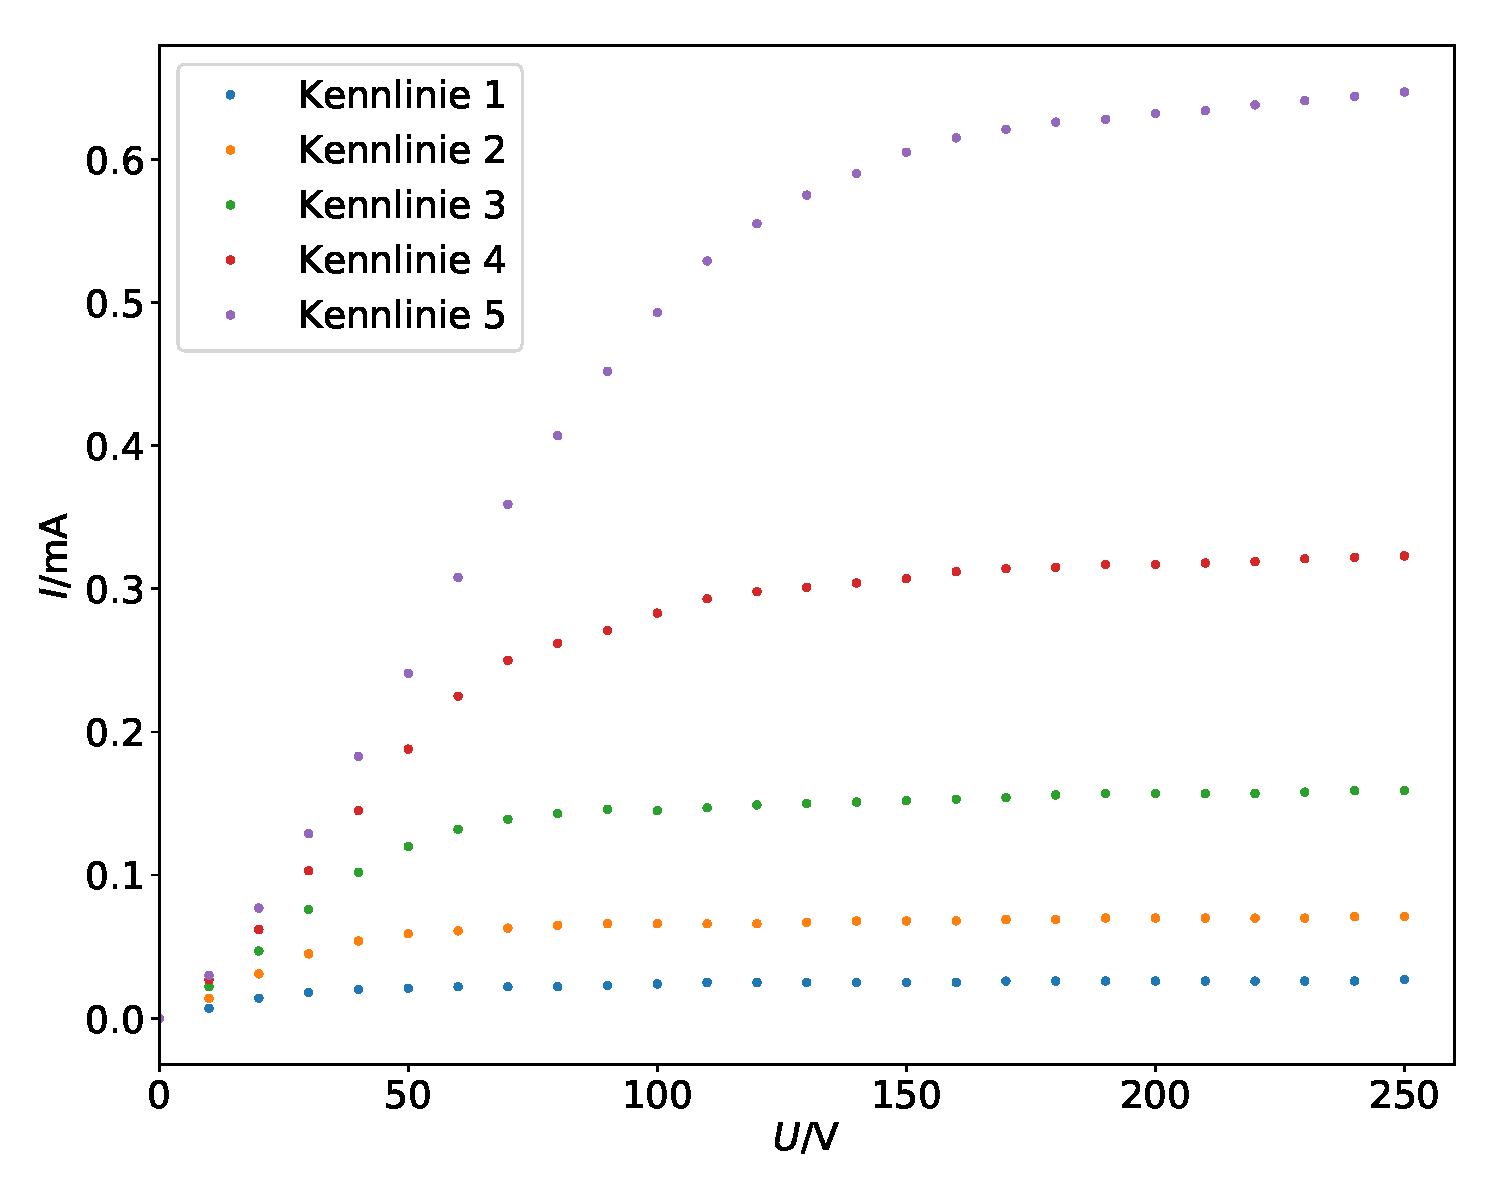
\includegraphics[scale=0.35]{kennlinien.pdf}
  \caption{Graphische Darstellung der Messwerte zur Bestimmung der Kennlinien.}
  \label{fig:1}
\end{figure}
Die Sättigungsströme sind die maximalen Werte aus Tabelle \ref{tab:1} und in Tabelle
\ref{tab:3} zu finden.
\begin{table}[h]
  \centering
  \caption{Heizspannungen und -ströme der Kennlinien aus Tabelle \ref{tab:1} mit den Sättigungsströmen.}
  \label{tab:3}
  \begin{tabular}{c c c}
    \toprule
    $U_{\symup{H}}$ / \si{\volt} & $I_{\symup{H}}$ / \si{\ampere} & $I_s$ / \si{\milli\ampere} \\
    \midrule
    3.0 & 1.8 & 0.027 \\
    3.5 & 1.9 & 0.071 \\
    4.0 & 2.0 & 0.159 \\
    4.2 & 2.1 & 0.323  \\
    4.7 & 2.2 & 0.647  \\
    \bottomrule
  \end{tabular}
\end{table}

\subsection{Bestimmung des Raumladungsgebietes}
Für die Messwerte $I_5$ wird das Raumladungsgebiet untersucht. Nach \eqref{eq:4} hat
dabei der Strom eine $V^{\frac{3}{2}}$ Abhängigkeit. Diese wird mittels linearer Regression untersucht.
Dazu werden die Spannung und der Strom logarithmiert und gegeneinander aufgetragen. Dies und die
Regression sind in Abbildung \ref{fig:2} zu sehen. Eine lineare Ausgleichsrechnung ergibt für
den Exponenten der Spannung \num{1.291(14)}.
\begin{figure}
  \centering
  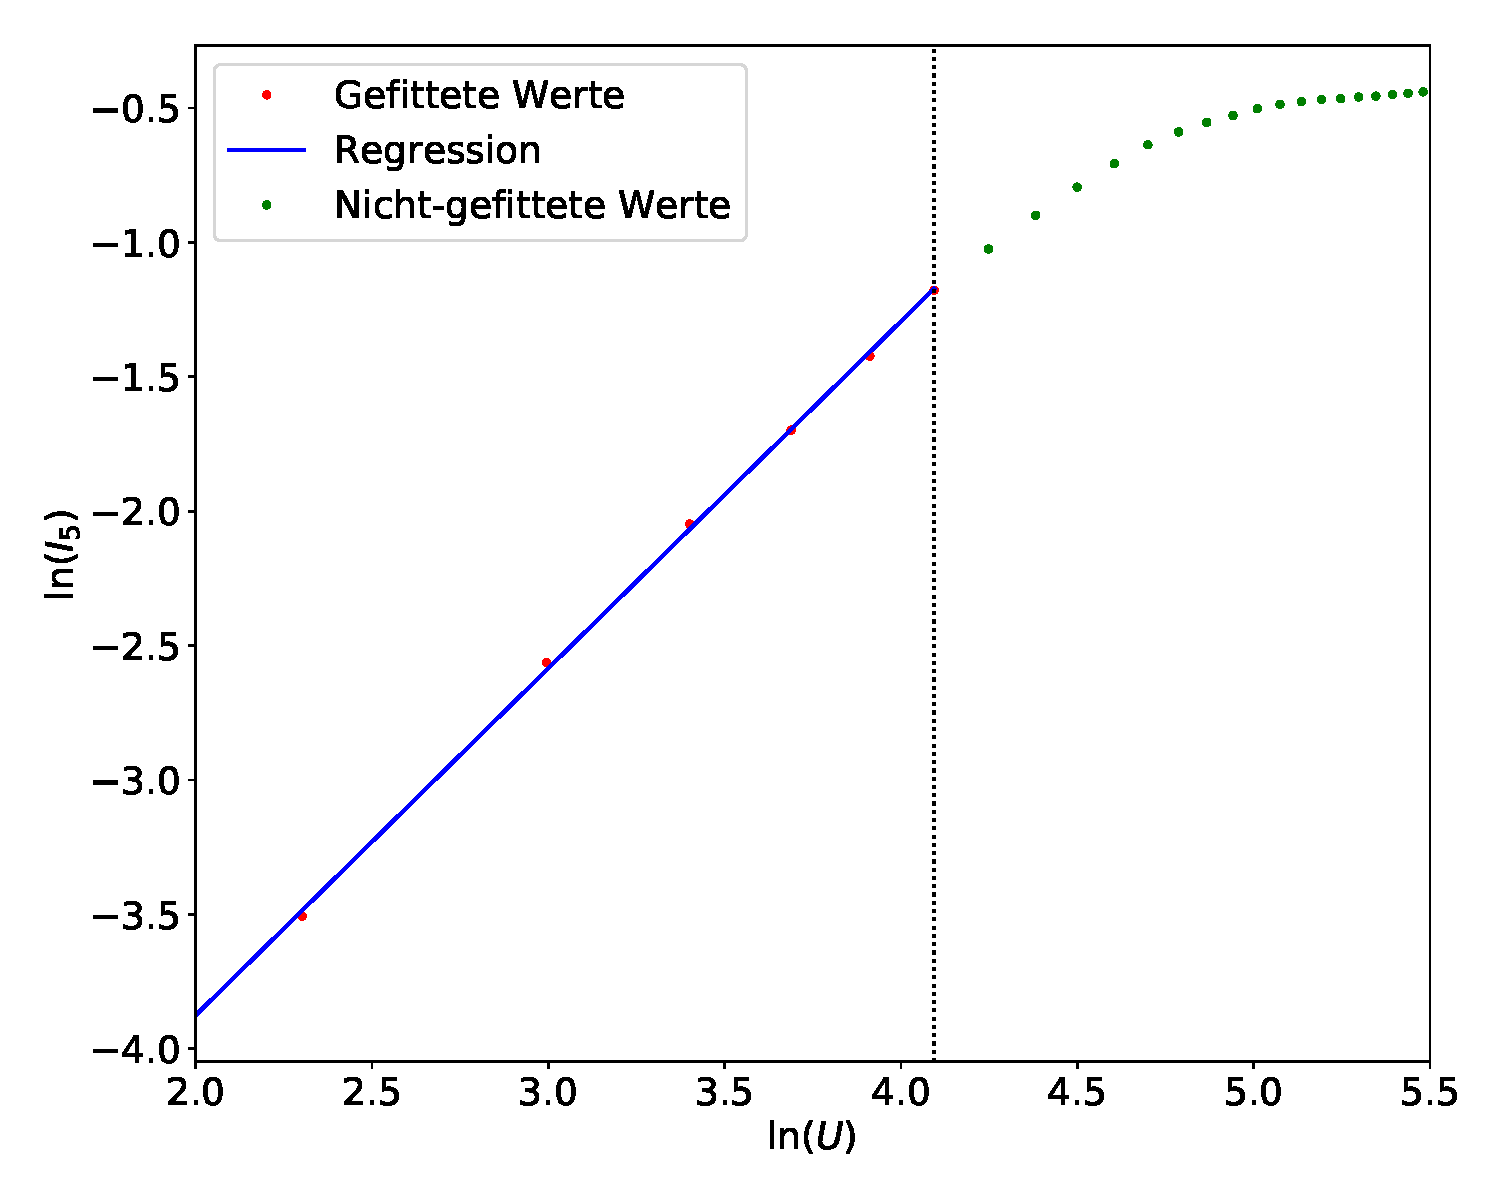
\includegraphics[scale=0.3]{raumladung.pdf}
  \caption{Graph zur Untersuchung des Raumladungsgebietes. Die gestrichelte Linie gibt an,
  bis wohin die $V^{\frac{3}{2}}$ Abhängigkeit gilt und somit bis zu welcher Spannung vom
  Raumladungsgebiet gesprochen werden kann.}
  \label{fig:2}
\end{figure}

\subsection{Untersuchung des Anlaufstromgebiets}
\label{sec:c}
Die Messwerte zur Kennlinie des Anlaufstromgebietes befinden sich in Tabelle
\ref{tab:2}.
\begin{table}[h]
  \centering
  \caption{Messwerte zur Kennlinie des Anlaufstromsgebiet.}
  \label{tab:2}
  \begin{tabular}{c c c}
    \toprule
    $U$ / \si{\volt} & $I_6$ / \si{\nano\ampere} & $U_{\symup{korr}}$ / \si{\volt} \\
    \midrule
    0.00 & 9.500 & -0.00950 \\
    0.10 & 5.000 & 0.09500 \\
    0.20 & 3.000 & 0.19700 \\
    0.30 & 1.600 & 0.29840 \\
    0.40 & 0.900 & 0.39910 \\
    0.50 & 0.500 & 0.49950 \\
    0.60 & 0.320 & 0.59968 \\
    0.70 & 0.200 & 0.69980 \\
    0.80 & 0.130 & 0.79987 \\
    0.90 & 0.125 & 0.89987 \\
    0.96 & 0.110 & 0.95989 \\
    \bottomrule
  \end{tabular}
\end{table}
Die grafische Darstellung ist in Abbildung \ref{fig:3} zu finden. Dabei wurden
die Ströme logarithmiert aufgetragen.
\begin{figure}[h]
  \centering
  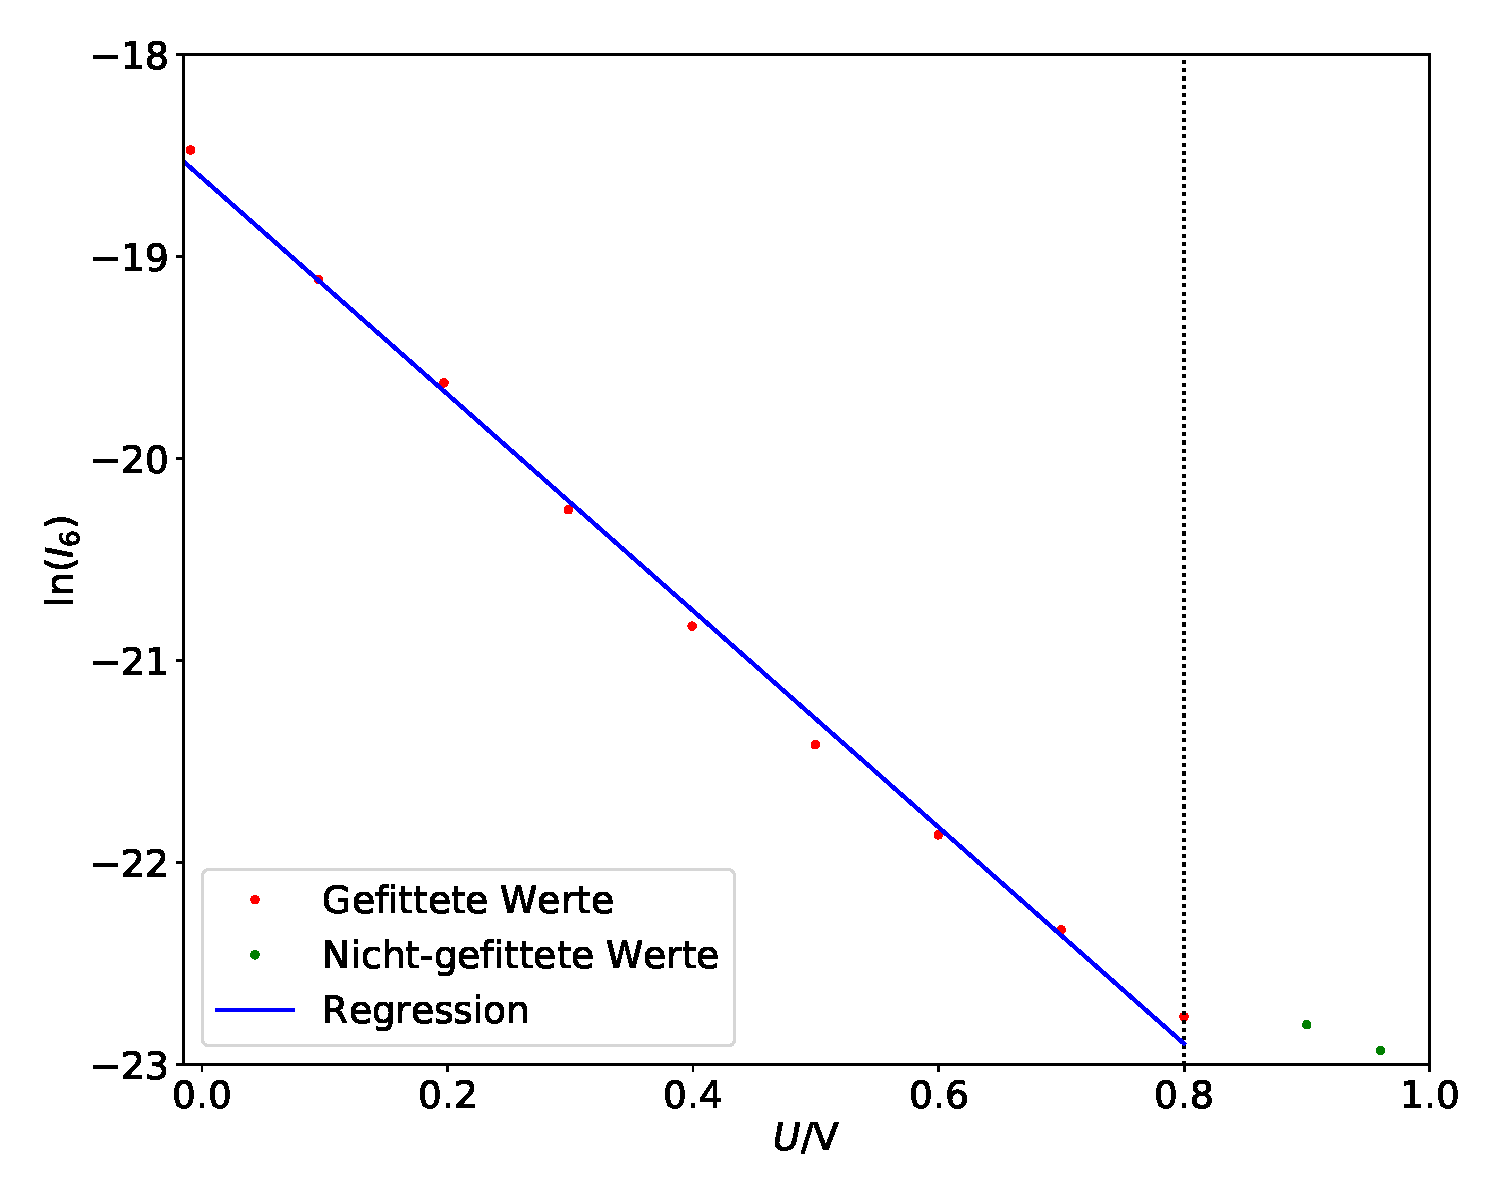
\includegraphics[scale=0.3]{anlauf.pdf}
  \caption{Graph zur Untersuchung des Anlaufstromgebietes. Die zwei Messwerte rechts von der
  gestrichelten Linie sind nicht in den Fit einbezogen worden, da sie nicht zu den restlichen Werten
  des Anlaufstromgebietes passen. Sie sind vermutlich durch Messrauschen entstanden.}
  \label{fig:3}
\end{figure}
Dabei ist zu beachten, dass die Spannung im Graph angepasst wurde,
da am Innenwiderstand des Amperemeters Spannung abfällt, siehe Abbildung \ref{abb:8}.
Die Spannungen sind in Tabelle \ref{tab:2} angegeben.
Mithilfe der Regression soll ein Ausdruck für die Kathodentemperatur $T$ gefunden
werden. Dazu wird \eqref{eq:5} umgestellt zu
\begin{equation*}
    \symup{ln}(I) = \symup{ln}(\symup{const}) - \frac{\symup{e}_0 \, U}{\symup k \cdot T} \, .
\end{equation*}
Die Steigung der linearen Regression gibt eine Wert für $\symup{e}_0/(\symup k \cdot T)$ an
und es folgt
\begin{equation}
    T = - \frac{\symup{e}_0}{\symup k \cdot x}
    \label{eqn:1}
\end{equation}
mit $x$ als Steigung der lienaren Regression. Aus \eqref{eqn:1} ergibt sich
$T = \SI{2.17(5)e3}{\kelvin}$.

\subsection{Temperaturbestimmung aus Leistungsbilanz}
Zur Erzeugung der Kennlinien aus Kapitel \ref{sec:a} werden die Heizspannungen und -ströme
aus Tabelle \ref{tab:3} genutzt.
Mit der Gleichung
\begin{equation}
    T = \left(\frac{U_{\symup{H}} \cdot I_{\symup{H}} - N_{\symup{WL}}}{\eta \, \sigma \, f} \right)^{\frac{1}{4}}
    \label{eqn:2}
\end{equation}
lassen sich Werte für $T$ finden. Diese folgt aus der Annahme, dass die zugeführte
elektrische Leistung in Form von Wärmestrahlung abgestrahlt und in Form von
Wärmeleitung abgegeben wird. Dabei ist $N_{\symup{WL}} = \SI{0.9}{\watt}$ die als Wärmeleitung abgegebene Leistung,
$\eta = \num{0.28}$ der Emissiongrad der Oberfläche, $\sigma$ = \SI[per-mode=reciprocal]{5.7e-12}{\watt\per\centi\meter\squared\per\kelvin\tothe{4}}
die Boltzmannsche Strahlungskonstante und $f = \SI{0.32}{\centi\meter\squared}$ die emittierende Kathodenoberfläche.
Da es fünf verschiedene Heizleistungen gibt, gibt es auch fünf verschiedene Temperaturen. Diese finden sich
in Tabelle \ref{tab:4}.
\begin{table}[h]
  \centering
  \caption{Temperaturen aus \eqref{eqn:2}.}
  \label{tab:4}
  \begin{tabular}{c c c c c}
    \toprule
    $T_1$ / \si{\kelvin} & $T_2$ / \si{\kelvin} & $T_3$ / \si{\kelvin} & $T_4$ / \si{\kelvin} & $T_5$ / \si{\kelvin} \\
    \midrule
    1722.89 & 1831.78 & 1930.94 & 1984.43 & 2073.47 \\
    \bottomrule
  \end{tabular}
\end{table}
Der Mittelwert ergibt sich zu $T = \SI{1.91(6)e3}{\kelvin}$.

\subsection{Bestimmung der Austrittsarbeit}
Aus den Sättigungströmen aus Kapitel \ref{sec:a} und den Temperaturen aus Tabelle \ref{tab:4}
lässt sich mit Formel \eqref{eq:3} die Austrittsarbeit berechnen. Dabei ist zu beachten, dass
$j_{\symup{S}} = I_{\symup{S}}/f$ gilt. \eqref{eq:3} wird umgestellt zu
\begin{equation}
  \symup{e}_0 \Phi = - \symup{ln}\left(\frac{I_{\symup{S}} \, \symup{h}^3}{4 \pi \, f \, \symup{e}_0 \, \symup{m}_0 \, \symup{k}^2 \, T^2} \right) \cdot \symup k T
  \label{eqn:3}
\end{equation}
Es ergeben sich mit \eqref{eqn:3} die Werte in Tabelle \ref{tab:5}.
\begin{table}
  \centering
  \caption{Austrittsarbeiten bei verschiedenen Temperaturen und Sättigungsströmen.}
  \label{tab:5}
    \begin{tabular}{c c c c c}
      \toprule
      $\symup e_0 \phi_1$ / \si{\electronvolt} & $\symup e_0 \phi_2$ / \si{\electronvolt} &
      $\symup e_0 \phi_3$ / \si{\electronvolt} & $\symup e_0 \phi_4$ / \si{\electronvolt} &
      $\symup e_0 \phi_5$ / \si{\electronvolt} \\
      \midrule
      4.32 & 4.46 & 4.58 & 4.60 & 4.69 \\
      \bottomrule
    \end{tabular}
\end{table}
Der Mittelwert der Austrittsarbeiten beträgt $\symup{e}_0 \Phi = \SI{4.53(7)}{\electronvolt}$.

\section{Diskussion}
Bei der Betrachtung der Ergebnisse zeigt sich, dass die Temperaturen, die aus dem Anlaufstrom
und aus der Heizleistungsbetrachtung gewonnen wurden, sich stark unterscheiden. Da allerdings
die Austrittsarbeit von Wolfram mit zweiterer Methode bestimmt wurde und diese vom Literaturwert\footnote{Siehe \cite{wolfram}}
\SI{4.54}{\electronvolt} nur 0.22\% abweicht (und innerhalb der Messungenauigkeit liegt), legt
dies den Schluss nahe, dass die Heizleistungsbetrachtung bessere Werte liefert als die Methode,
die Temperatur mithilfe des Anlaufstromgebietes zu untersuchen. Erklären lässt sich das damit,
dass in Kapitel \ref{sec:c} Ströme im \si{\nano\ampere}-Bereich gemessen werden, welche
schwierig exakt zu bestimmen sind.

Die Bestimmung des Raumladungsgebietes und die Verifizierung der Gültigkeit des
Langmuir-Schottkyschen Raumladungsgesetzes ist alles in allem eher schlecht verlaufen. Der
gemessene Wert liegt nicht innerhalb der Messungenauigkeit, die relative Abweichung beträgt 13.93\%.
Allerdings ist die Abweichung des Fehlerintervalls mit $15 \sigma$ ziemlich groß. Die Ursache dafür liegt ihrer endlichen Größe
und in der Bauart der Anode,
die nicht alle von der Kathode emittierten Elektronen aufnehmen kann.
\newpage
\nocite{*}
\printbibliography
